\documentclass{beamer}

\usepackage[utf8]{inputenc}
\usepackage{tikz}
\usepackage{multirow}
\usepackage{pgfplots}

\title{Mushroom classification\\
with MobileNetV2 and Xception}
\author{Lorenzo Vainigli\\
lorenzo.vainigli@studio.unibo.it\\
matr. 0000842756}
\institute{Course of Machine Learning\\
Laurea Magistrale in Informatica\\
University of Bologna}
\date{A.Y. 2020-2021}


\begin{document}

\frame{\titlepage}

\begin{frame}
\frametitle{Introduction}
\begin{itemize}
\setlength\itemsep{1em}
\item Purpose of the project: study and build a classifier that is
able to recognize images of mushorooms and categorieze them.
\item MobileNetV2
\begin{itemize}
\item 71\% in top-1 accuracy and 90\% in top-5 accuracy on ImageNet. 
\end{itemize}
\item Xception
\begin{itemize}
\item 79\% in top-1 accuracy and 95\% in top-5 accuracy on ImageNet. 
\end{itemize}
\item MobileNetV2 is six times smaller than Xception in memory
storage.
\end{itemize}
\end{frame}

\begin{frame}
\frametitle{Methods (2)}
\begin{block}{Software}
\begin{itemize}
\setlength\itemsep{1em}
\item Google Colab platform with Google GPUs; Tensorflow, Keras.
\end{itemize}
\end{block}
\begin{block}{Dataset}
\begin{itemize}
\setlength\itemsep{0.5em}
\item Each image has a label defined by the pair \textit{(super-category, category)}.
\item This dataset contains about 90,000 images belonging to about 1,500 classes.
\item For our work we used 6,739 images belonging to 20 classes.
\item To balance the dataset we picked:
\begin{itemize}
\item 414 images if we use the first 3 classes, 
\item 340 images if we use the first 10 classes;
\item 255 if we use all the 20 classes.
\end{itemize}
\end{itemize}
\end{block}
\end{frame}


\begin{frame}
\frametitle{Methods (3)}
\begin{figure}[h]
	\centering
    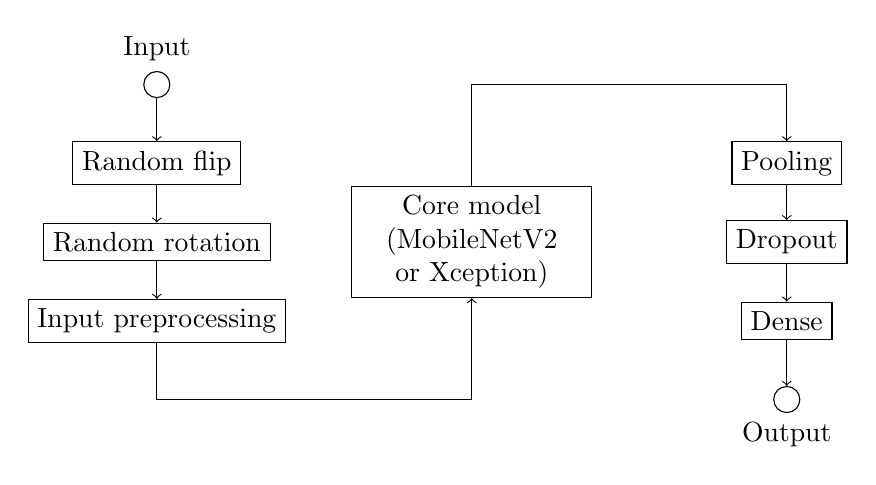
\begin{tikzpicture}
    \node[draw,circle,minimum size=3pt,label=above:Input] at (0,1) (in) {};
    \node[draw] at (0,0) (rf) {Random flip};
    \node[draw] at (0,-1) (rr) {Random rotation};
    \node[draw] at (0,-2) (pp) {Input preprocessing};
    \node[draw,text width=80pt,align=center] at (4,-1) (m) {Core model\\(MobileNetV2 or Xception)};
    \node[draw] at (8,0) (po) {Pooling};
    \node[draw] at (8,-1) (dr) {Dropout};
    \node[draw] at (8,-2) (de) {Dense};
    \node[draw,circle,minimum size=3pt,label=below:Output] at (8,-3) (out) {};
    \draw[->] (in.south) -- (rf.north) node {};
    \draw[->] (rf.south) -- (rr.north) node {};
    \draw[->] (rr.south) -- (pp.north) node {};
    \draw[->] (pp.south) -- (0,-3) -| (m.south) node {};
    \draw[->] (m.north) --  (4,1) -| (po.north) node {};
    \draw[->] (po.south) -- (dr.north) node {};
    \draw[->] (dr.south) -- (de.north) node {};
    \draw[->] (de.south) -- (out.north) node {};
    \end{tikzpicture}
    \caption{Architecture of the model.}
\end{figure}
\end{frame}

\begin{frame}
\frametitle{Methods (4)}
\begin{block}{Fine tuning}
\begin{enumerate}
\setlength\itemsep{1em}
\item First training phase: convolutional layer weughts update was disabled, only the final dense layer was updated.
\item Second training phase: also some convolutional layers were updated.
\end{enumerate}
\end{block}
\begin{block}{Hyperparameters}
\begin{itemize}
\setlength\itemsep{0.5em}
\item Split training - test = 80\%-20\%
\item Split training - validation = 80\%-20\%
\item Batch size = 32
\item Learning rate = $10^{-4}$ for phase 1, $10^{-5}$ for phase 2
\item Epochs = 100 for phase 1, 20 for phase 2  
\end{itemize}
\end{block}
\end{frame}

\begin{frame}
\frametitle{Results}
\begin{table}[h]
\centering
\setlength{\tabcolsep}{5pt}
\def\arraystretch{1.2}
\begin{tabular}{ |c|c|c|c|c|c| } 
 \hline
 \multirow{2}{4em}{\textbf{Classes}} & \multirow{2}{6em}{\textbf{Samples per class}} & \multicolumn{2}{|c|}{\textbf{MobileNetV2}} & \multicolumn{2}{|c|}{\textbf{Xception}} \\ 
 \cline{3-6}
 & & \textbf{Top-1} & \textbf{Top-5} & \textbf{Top-1} & \textbf{Top-5} \\
 \hline 
 3 & 414 & 92\% & - & 90\% & - \\ 
 \hline 
 10 & 340 & 77\% & 98\% & 81\% & 98\% \\
 \hline 
 20 & 255 & 65\% & 95\% & 70\% & 95\% \\
 \hline
\end{tabular}
\caption{Result values for top-1 accuracy and top-5 accuracy.}
\end{table}
\end{frame}

\begin{frame}
\frametitle{Results (2)}
\begin{figure}[h]
\centering
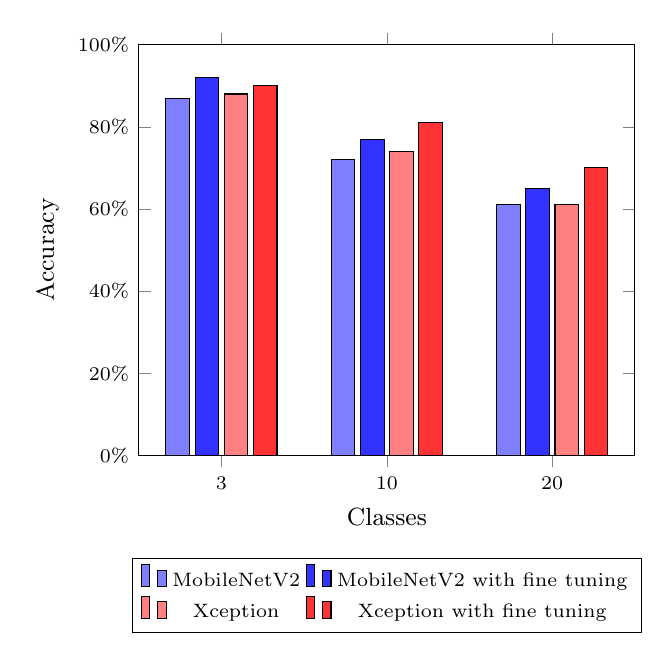
\begin{tikzpicture}
\begin{axis}[
	bar width=25,enlarge x limits=0.25,
	x tick label style={
        /pgf/number format/1000 sep=},
    ylabel={\small{Accuracy}},
    xlabel={\small{Classes}},
    yticklabel={\pgfmathparse{\tick}\pgfmathprintnumber{\pgfmathresult}\%},
    ymin=0,ymax=100,
    width = 0.65*\textwidth,
    legend style={
    	font=\scriptsize,
        at={(0.5,-0.25)},anchor=north
    },
    legend columns=2,
    symbolic x coords={3,10,20},
    xtick=data,
    tick label style={font=\scriptsize},
    ybar,
    bar width = .3cm
]
\addplot [fill=blue!50] coordinates {(3,87)(10,72)(20,61)};
\addplot [fill=blue!80] coordinates {(3,92)(10,77)(20,65)};
\addplot [fill=red!50] coordinates {(3,88)(10,74)(20,61)};
\addplot [fill=red!80] coordinates {(3,90)(10,81)(20,70)};
\legend{MobileNetV2,MobileNetV2 with fine tuning,Xception,Xception with fine tuning}
\end{axis}
\end{tikzpicture}
\caption{Comparison of performances between MobileNetV2 and Xception.}
\end{figure}
\end{frame}

\begin{frame}
\frametitle{Discussion}
\begin{itemize}
\setlength\itemsep{1em}
\item We notice that with increasing the number of classes,
the accuracy tends to decrease rapidly.
\item Comparing the the 1000 classes of ImageNet, 20 classes are very few.
\item Results probably will be better if:
\begin{itemize}
\item we have more samples for each class;
\item we extend the training phase with more epochs.
\end{itemize}
\end{itemize}
\begin{block}{Further directions}
\begin{itemize}
\item Try different setting for hyperparameters.
\end{itemize}
\end{block}
\end{frame}

\begin{frame}
\frametitle{Conclusions}
\begin{itemize}
\setlength\itemsep{1em}
\item A method to use pre-trained neural networks to classify mushrooms was presented. 
\item Dataset was explored and prepared.
\item The model was implemented following the offcial guidelines. \item A fine tuning phase was performed to achieve better performances. 
\item Results shows that models can correctly predict with noticeable accuracy.
\end{itemize}
\end{frame}

\end{document}